% WIP-Stil LaTeX-Vorlage für (englischsprachige) Abschluss- und Studienarbeiten

\documentclass[
	11pt,								% Schriftgroesse
	DIV10,								% Koma-Script-Klassen: Groesse des bedruckbaren Bereichs
	a4paper,         					% Format
	oneside,							% Einseitiges Dokument
	headheight=20pt,					% Höhe Dokumentenkopf
	footheight=20pt,					% Höhe Dokumentenfuß
    parskip=full,						% Abstand zwischen Absaetzen (ganze Zeile)
    listof=totoc,						% Verzeichnisse im Inhaltsverzeichnis aufführen
	bibliography=totoc,					% Literaturverzeichnis im Inhaltsverzeichnis aufführen
	index=totoc,						% Index im Inhaltsverzeichnis aufführen
	%final
    %draft								% Status des Dokuments
]{scrartcl}

%%% Schrift %%%
\usepackage[utf8]{inputenc}				% Umlaute im Tex-Code erlauben
\usepackage[T1]{fontenc}
\usepackage[ngerman, english]{babel}	% Sprachpaket Deutsch
\usepackage[useregional]{datetime2}
\selectlanguage{english}
\usepackage{csquotes}					% Zitation im gleichen Stil 
\renewcommand{\baselinestretch}{1.50}	% Zeilenabstand 1.5
\normalsize
%\usepackage{uarial}						% Schriftart Arial, kann ausdokumentiert werden, wenn die Standardschrift benutzt werden soll
\renewcommand{\familydefault}{\sfdefault}
\usepackage{blindtext}					% zum Testen des Layouts
\usepackage{microtype}					% Verbesserter Randausgleich
\usepackage{color}
\usepackage{eurosym} 					% Eurozeichen
\usepackage{xcolor}
\usepackage{datetime}
\usepackage{dcolumn}
\usepackage{todonotes}
\usepackage{eurosym}
\usepackage{amssymb}

%%% Anpassung des Formats %%%
\RedeclareSectionCommand[
  beforeskip=-1sp,						% minimaler Abstand nach Überschrift, anschließend nicht einrücken
  afterskip=1sp]{section}
\RedeclareSectionCommand[
  beforeskip=-1sp,						% siehe oben 
  afterskip=1sp]{subsection}
\RedeclareSectionCommand[
 beforeskip=-1sp,						% siehe oben
  afterskip=1sp]{subsubsection}
\RedeclareSectionCommand[
  beforeskip=-1sp,						% siehe oben
  afterskip=1sp]{paragraph}
\RedeclareSectionCommand[
 beforeskip=-1sp,						% siehe oben
 afterskip=1sp]{subparagraph}

%%% Änderungen des Inhaltsverzeichnis %%%
\usepackage[titles]{tocloft}			% wird zur Änderung des toc verwendet

\renewcommand{\cftsecleader}			% führe Punkte im toc auch für sections ein, Punkte fetter als normal
	{\bfseries\cftdotfill{\cftdotsep}}
\renewcommand{\cftdotsep}{0.1}			% setze Punkteabstand enger	

%%% definiere Inhaltsübersicht %%%
% Achtung: In Vorlage auskommentiert %
\newcommand*\inhaltsuebersicht{%
\section*{Content Overview}				% Name 
\begingroup
\value{tocdepth}\shorttocdepth\relax
\makeatletter
\input{\jobname.toc}
\makeatother
\endgroup
}
\newcommand*{\shorttocdepth}{1}			% Tiefe der Inhaltsübersicht == 2

%%% Bilder %%%
\usepackage{graphicx}
\graphicspath{{./Bilder/}}				% Bilderverzeichnis
\usepackage{overpic} 					% Beschriftung in Abbildung platzieren
\usepackage{here}						% Bildplatzierung mit [H]

%%% Verschiedenes, Mathe-Funktionen, Layout %%%
\usepackage{float,caption}
\usepackage{amsmath,amsfonts}
\usepackage{mathtools}
\usepackage{amssymb}
\usepackage{exscale}
\usepackage[normalem]{ulem}
\usepackage{setspace}
\usepackage[a4paper,
    lmargin={2.5cm},
    rmargin={2.5cm},
    tmargin={2cm},
    bmargin={2cm}
    ]{geometry}
    
\addtolength{\footskip}{-0.5cm}			% Fussbereich 0.5cm höher, sodass die Seitennummierung höher ist

%%% Listen %%%
%\usepackage{enumitem}
\usepackage{paralist}					% Für kompakte Listen
\setlength{\pltopsep}{5pt}				% setzt den oberen Abstand der compactitem- und compactenum-Liste auf eine Zeilenbreite

%%% Tabellen %%%
\usepackage{tabularx}
\usepackage{booktabs}					% Platzverschwendung in Tabellen vermeiden
\usepackage{array}						% mehr Möglichkeiten der Darstellung

%%% Kopf und Fußzeile %%%
\usepackage[nouppercase,headsepline]{scrpage2}
\pagestyle{scrheadings}
\clearscrheadfoot
%\chead{\textit{TU Berlin, Fachgebiet Wirtschafts- und Infrastrukturpolitik (WIP)}}
	% Leerzeichen zwischen FN-Nummer und FN-Text
\deffootnote[]{1.5em}{1em}{\textsuperscript{\thefootnotemark}\enskip}
\cfoot{\normalsize{\emph{\thepage}}}

%%% URL's %%%
\usepackage[lowtilde]{url}				% bei Verwendung eines Tildezeichens wird es normal gesetzt
\urlstyle{same}
\usepackage{etoolbox}

%%% Zitation %%%
\usepackage[%style=chicago-authordate,
			%style=authoryear,
			style=nature,
            giveninits,					% Vornamen abkürzen
			maxbibnames=10,				% in der Bib werden 10 Autoren ausgegeben (bis zu 10)
            maxcitenames=2,				% max. 3 Autoren bei \cite
            backend=biber,
			doi=false,
			isbn=false,
			url=false,
            natbib=true,				% verwendet Natbib 
            sorting=nyt					
			]{biblatex}

\addbibresource{microgrid_literature.bib}
\addbibresource{extra_literature.bib}
\usepackage{breakcites}

\DeclareNameAlias{author}{last-first}				

% *****************************************
%%% Anpassungen für englische Literatur %%%
% *****************************************

\DeclareFieldFormat[article]{title}{"#1\adddot"}				
\DeclareFieldFormat[inproceedings]{title}{"#1\addcomma"}				
%\DeclareFieldFormat[book]{title}\textit{{#1}\isdot}    			
\DeclareFieldFormat[techreport]{title}{"#1\adddot"}					
\DeclareFieldFormat[incollection]{title}{"#1\adddot"} 
\DeclareFieldFormat[online]{title}{#1\isdot}           		
\DeclareFieldFormat[misc]{title}{"#1\isdot"}					

\DeclareFieldFormat[inproceedings]{booktitle}{proceedings of #1}	

\AtEveryBibitem{\clearlist{language}}

\AtEveryBibitem{%
	\ifentrytype{online}
	{}
	{\clearfield{urlyear}\clearfield{urlmonth}\clearfield{urlday}}}

\AtEveryBibitem{%
	{\clearfield{month}\clearfield{day}}}

\DefineBibliographyStrings{english}{andothers = {et\,al\adddot}}

\DeclareFieldFormat[article]{number}{#1}					
\DeclareFieldFormat[article]{pages}{\space#1}

\usepackage{xpatch}
\xpretobibmacro{author}{\mkbibbold\bgroup}{}{}					% Autor fett
\xapptobibmacro{author}{\egroup}{}{}

\DeclareSourcemap{
	\maps{\map{
			\step[fieldsource=language, fieldset=langid, origfieldval, final]
			\step[fieldset=language, null]}}}

\usepackage[pdfborder={0 0 0},								% Rahmen in pdf nicht sichtbar
			breaklinks=true,
            %draft,											% alle Links abschalten
            ]{hyperref}

%%%%%%%%%%%%%%%%%%%%%%%%%%%%%%%%%%%%%%%%%%%%%%%%%%%%%%%%%%%%%%%%%%%%%%%%%%%%%%%%%%%%%%%%%%%%%%%
% Beginn des Dokument

% *************************************
%%% HIER DIE TITELSEITE BEARBEITEN %%%%
% *************************************

%%% Titelseite %%%
\newcommand{\autor}{Maximilian Eißler} 		% Name des Autors
\newcommand{\matriculation}{374881} 
\newcommand{\mailaddress}{eissler@campus.tu-berlin.de}

\newcommand{\betreuer}{Dr. Pao-Yu Oei} 		% Namen der Betreuer
\newcommand{\betreuerzwei}{Thorsten Burandt}
                      
                  
%\newcommand{\datum}{\selectlanguage{ngerman}\today}
\newcommand{\engdate}{\selectlanguage{english}\today}

%%% Glossar und Abkürzungsverzeichnis %%% 
\usepackage[acronym,
            nonumberlist,									% keine Seitenzahlen anführen
            toc,											% im Inhaltsverz. mit aufnehmen
            style=super,									% Einträge mit Abstand setzten 
            nopostdot,										% kein schließender Punkt
           	nogroupskip]									% kein Absatz zwischen Gruppen
           	{glossaries}									% muss nach \usepackage{hyperref} geladen werden, damit auch Einträge des Abkürzungsverzeichnisses verlinkt sind
\makeglossaries

%***********************************
%%% HIER DIE AKRONYME DEFINIEREN %%%
%***********************************

%%% exempl. Akronyme %%%
\newacronym[firstplural=renewable energy sources (RES)]{res}{RES}{renewable energy sources}
\newacronym{eeg}{EEG}{Erneuerbare-Energien-Gesetz}
\newacronym{tso}{TSO}{Transmission System Operator}
\newacronym{rmse}{RMSE}{root-mean squared error}
\newacronym{gams}{GAMS}{General Algebraic Modeling System}
\newacronym[firstplural=Energiewirtschaftsgesetzes (EnWG)]{enwg}{EnWG}{Energiewirtschaftsgesetz}
\newacronym{ihv}{i.H.v.}{in Höhe von}
\newacronym[firstplural=Millimetern (mm)]{mm}{mm}{Millimeter}
\newacronym[firstplural=Off\-shore-Wind\-parks (OWP)]{owp}{OWP}{Off\-shore-Wind\-park}
	% sort= ermöglicht korrekte Sortierung von Umlauten
\newacronym[sort=uebertr]{unb}{\"UNB}{Übertragungsnetzbetreiber}

% ***********************************************************************************
% Beginn des Dokuments
% ***********************************************************************************

\begin{document}\selectlanguage{english}
% ***********************************************************************************
% Automatische Zusammensetzung der Titelseite, nur aendern, falls noetig!
% ***********************************************************************************

	\thispagestyle{plain}
	\begin{titlepage}
		\vspace{0cm} 
		\begin{center}
			
\includegraphics[width=2.5cm]{pictures/TU_Logo_kurz_4c_rot}\\
			\normalsize{Technische Universität Berlin}\\
			Fakultät VII Wirtschaft \& Management\\
			Fachgebiet Wirtschafts- und Infrastrukturpolitik (WIP)
		\end{center}
        \vfill
		%\vspace*{\fill}
		\begin{center}
			%\Large{\textbf{\textsc{\doctitle}}}\\
			\Large{\textbf{Bachelorarbeit}}\\
            \LARGE{\textbf{Title}}\\[2ex]
            \Large{\textbf{Subtitle}}
            
			\vfill
			
% "Ockerfarbener Kasten":

%{
%\setlength{\fboxrule}{0.2mm}
%\definecolor{ocker}{RGB}{196,188,150}
%			\selectlanguage{ngerman}\normalsize
%\fcolorbox{black}{ocker}{\begin{minipage}{\textwidth}

%\textbf{Dateinamen-Kern (mit Versions-Nr. 000):} 
%\url{vorlage_latex_v000}

%\textbf{Ablage-Server-Pfad (fixiert):} 
%\url{Z:\\lehre\\BEREICH_WIPOL_ETC\\veranstaltung___ewa_seminar\\_formatvorlagen\\LaTeX-Vorlagen\\Standard}

%\textbf{Aktueller Ablageort:} \url{\\\\afs\\tu-berlin.de\\units\\Fak_VII\\wip\\share\\lehre\\BEREICH_WIPOL_ETC\\veranstaltung___ewa_seminar\\_formatvorlagen\\LaTeX-Vorlagen\\Standard\\vorlage_latex_v001_vc_17-05-2017}

%\textbf{Datum:} \today \ \currenttime
%\end{minipage}}}

			\vfill
			\normalsize
			Author(s): \\
			\autor \, (\matriculation) - \mailaddress \\
            \vfill
			Supervisors:\\\betreuer	\\
			\betreuerzwei
			%\vspace*{\fill}
            \vfill
			Berlin, \engdate
		\end{center}
		
	\end{titlepage}
	\newpage
	\pagenumbering{roman}
	
% ***********************************************************************************
% Eidesstattliche Erklaerung, automatisch generiert
% ***********************************************************************************


\setcounter{page}{2}							% Seitenzahl == 2 (Titelseite wird mitgezählt)
% \chead{\textit{Eidesstattliche Erklärung}}
% \section*{Eidesstattliche Erklärung}
%	
%	Hiermit erkläre ich, \autor, an Eides statt, dass ich die vorliegende Arbeit selbstständig und nur unter Zuhilfenahme der ausgewiesenen Hilfsmittel angefertigt habe.\\
%	Sämtliche Stellen der Arbeit, die im Wortlaut oder dem Sinn nach anderen gedruckten oder im Internet verfügbaren Werken entnommen sind, wurden durch genaue Quellenangaben kenntlich gemacht.
%
%	

\chead{\textit{Statutory declaration}}
\section*{Statutory declaration}
	Hereby, I declare that I have developed and written this research completely by myself and that we have not used sources or means without declaration in the text. Any external thought, content, media, or literal quotation is explicitly marked and attributed to its respective owner or author. \\
	As of the date of submission, this piece of doument and its content have not been submitted anywhere else but to our supervisors.
	
	\bigskip
	
	Berlin, \engdate
	
	\bigskip
	\bigskip
		\begin{center}	
			\begin{minipage}[t]{0.3\textwidth}
				\rule[-0.2cm]{4.5cm}{0.5pt} \\
				\textsc{\autor}
			\end{minipage}
		\end{center}
	
	\newpage

% ****************************	
% Abstract und ggf. Zusammenfassung
% ****************************

	\chead{\textit{Abstract}}
	\section*{Abstract}
	
	Lorem ipsum dolor sit amet, consetetur sadipscing elitr, sed diam nonumy eirmod tempor invidunt
	ut labore et dolore magna aliquyam erat, sed diam voluptua. At vero eos et accusam et justo
	duo dolores et ea rebum. Stet clita kasd gubergren, no sea takimata sanctus est Lorem ipsum
	dolor sit amet. \\
	Lorem ipsum dolor sit amet, consetetur sadipscing elitr, sed diam nonumy eirmod tempor invidunt
	ut labore et dolore magna aliquyam erat, sed diam voluptua. At vero eos et accusam et justo
	duo dolores et ea rebum. Stet clita kasd gubergren, no sea takimata sanctus est Lorem ipsum
	dolor sit amet.
	
	\newpage	

% ***********************************************************************************
% Verzeichnisse
% ***********************************************************************************
	\selectlanguage{english}	
	
	\chead{\textit{Index}}
	\setcounter{tocdepth}{4} 					% Tiefe des Inhaltsverzeichnisses
    \setcounter{secnumdepth}{4}					% Tiefe der gezählten Überschriften
	
    \begingroup									% verringere Abstände in der Inhaltsübersicht
	\parskip=0pt	
    \endgroup
    \newpage
    \begin{onehalfspace}
    \chead{\textit{Contents}}
    \tableofcontents 							% Inhaltsverzeichnis
	\end{onehalfspace}
	\newpage
	\setkomafont{captionlabel}{\bfseries}
	\setkomafont{caption}{\bfseries}			% Bild- und Tabellenbeschriftung fett
		
	% Vor der Zahl steht Figure im Verzeichnis
	\renewcommand{\cftfigpresnum}{Figure }
	\settowidth{\cftfignumwidth}{Figure 5\quad}  
	\listoffigures								% Abbildungsverzeichnis
	%\newpage
		
	% Vor der Zahl steht Table im Verzeichnis
	\renewcommand{\cfttabpresnum}{Table }
	\settowidth{\cfttabnumwidth}{Table 150\quad}
	\newpage
	\listoftables								% Tabellenverzeichnis
	% \newpage
	%
	% %Glossary/List of Acronyms
	% \printglossary								% Glossar
	% \newpage
	% \printglossary[type=\acronymtype,			% Akronyme und Abkuerzungen
    %				title={List of Acronyms}]
    \newpage
	\pagenumbering{arabic}						% beginne mit "normaler" Nummerierung
	
% ***********************************************************************************
% CHEATSHEET
% Acronyms: \gls{tso}; \gls{gams}
%
%Chicago (author-date) citation style is used.\\
%In-text citation:
%\citet{abrell_integrating_2015} employed...
%
%Other forms of citation:
%.... (see \citealt{birge_introduction_2011})
%Please maintain a consistent table style (booktabs). For convenience, feel free to use a \href{https://www.tablesgenerator.com/}{TeX table generator}.
%\begin{table}[H]
%	\centering
%	\caption{An exemplary table}
%	\begin{tabular}{lll}
%		\hline
%		\textbf{First Column}		   & \textbf{Second Column}     & \textbf{Third Column}       \\ \hline
%		First Row                      & information     			& information     \\
%		Second Row                     & information     			& information     \\
%		Third Row					   & information     			& information     \\ \hline
%	\end{tabular}
%\end{table}
%\begin{flushleft}
%	\quad\quad\footnotesize{Source: Based on \citet{leuthold_large-scale_2012}.}
%\end{flushleft}
%\begin{figure}[H]
%	\centering
%	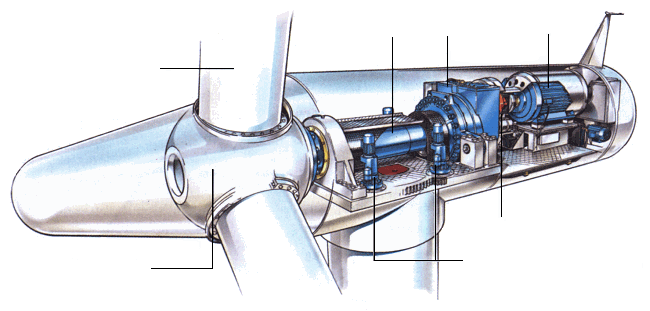
\includegraphics[width=\textwidth]{pictures/wind_turbine.png}
%	\caption{An exemplary figure}
%	\label{wind_turbine}
%	\flushleft\quad\quad\footnotesize{Source: Own illustration.}
%\end{figure}	
% ***********************************************************************************
	
% ***********************************************************************************
% Beginn des eigenstaendigen Teils
% ***********************************************************************************

\selectlanguage{english}


\chead{\textit{Introduction}}					% definiere Kopfzeile
%\include{files/Introduction}					% include statt input ermöglicht Arbeit mit \includeonly{} und fügt Seitenumbruch vor section ein

\section{Introduction}
In this document the topic, motivation and approach of my bachelor’s thesis shall be outlined. The aim is to give the reader an idea of what I try to accomplish with the choice of topic and methods, as well as a look at the first iteration of the mathematical model I am aiming to build.

\subsection{Motivation}
As the technological requirements for a decentralized energy system increasingly mature, the importance of understanding smaller units within the electricity system grows. There is a possibility of increasing reliance on small, partially autonomous grid units (microgrids) in the future. This calls for a better understanding of how such systems might operate. Especially the possible efficiency gains over a centralised system and the circumstances on which these efficiency gains might depend should be of interest to science and will be the focus of thesis.

\subsection{Research Question}
In my thesis I want to create a model of a small electricity grid with a single point of access to the main grid. The microgrid will contain 25 households of different types that will aim to reduce their total electricity costs. To attain this goal there will be two possible courses of action available: 
	\begin{enumerate}
	\item First, the option to invest in electricity generation and storage facilities, in this case only solar pv and battery storage. 
	\item Secondly, the possibility of unrestricted trade within the microgrid, meaning there will be no variable transaction costs, as they would usually occur in the form of fees and levies on electricity being transferred.		
	\end{enumerate}
	The aim of this approach is to determine the cost-saving potential in comparison to pure electricity consumption from the main grid in subject to the characteristics of the main parameter types to this model, which are:
	\begin{enumerate}
	\item The environmental conditions, primarily pertaining to the availability of renewable resources - in this case, solar irradiation - as well as temperature and changing seasonal energy demand.
	\item The 'behaviour' of the participants in this microgrid, primarily their willingness to shift or avoid loads depending on the current price of electricity within the microgrid or the main grid.
	\item The price of power from the main grid as a function of the time of day and  season, as well as the price of power generated by the households themselves.
	\end{enumerate}

\subsection{Methods}
	To model the outlined situation I want to use the computational modelling language 'Julia' and construct a linear optimisation model which can be solved with it. The goal is to minimise the cost of electricity for the households in the microgrid. It is notable at this point, that the non-consumption of electricity as well as the delay of consumption will be seen as a cost to the actor forgoing her demand. There will be an investment opportunity at the beginning of the examined timeframe of 20 years. The number of timeslices considered in the optimisation will be depending on performance of the model and can therefore not be determined yet. \\
	As a case study for this thesis I want to apply the model to the example of a community in Northrhine-Westfalia. With environmental variables set, I will then construct a number of scenarios with variations in electricity price and actor behaviour parameters. \\
	Another goal of this project is to make this a functional piece of research by reducing performance requirements as far as possible and creating an intuitive user interface that enables the user to 'play' with different scenarios. I prefer this approach over a few detailed and rigid scenarios because the future external factors are presently highly uncertain, which drives me to the conviction that an understanding of the dynamics involved in the examined system is of greater value than an exact solution to an unlikely scenario.
	
\subsection{Expected Results}
The result should be a tool that enables an intuitive understanding of the characteristics and the potentials of microgrids, even to non-economists. I intend an exemplary application of the model to the case of a Northrhine-Westfalian community. From this application I expect an insight into the efficiency gains achievable by microgrids in the German context. Also the required external factors for these efficiency gains to materialise should become evident. Under the right conditions I expect a double digit percentage drop in electricity costs compared to a purely consumption-based system. I hope to arrive at practical conclusions regarding present use cases for microgrids and required future regulation.
\newpage

\section{Literature Review}
In this section I shall attempt to give an overview over the current status quo regarding the optimizaton of microgrids and more especially the tools available to do so. I will pursue  this by answering a number of broad question, which I think are crucial regarding my subject. The procedure will be structured by utilizing a consistent and reproducible methodology described in detail below. In addition to scientific literature other sources will also be taken into account at my discrection if they are neccessary or helpful in answering a question.

\subsection{Key Questions}
This literature review will attempt to answer the following key questions in the context of my subject:
\begin{enumerate}
	\item What are the most eminent scientific standards for modelling a microgrid allocation and dispatch?
	\item What is usually within the scope of such a model (what types of generation assets, only electricity or also thermal energy and so on)? 
	\item What are the common methods used to determine some of the key variables required in such a model such as interest rates, CAPEX and OPEX of assets and so on?
	\item What are the most commonly used (commercial) tools for optimizing a microgrid? Are there any free or open source solutions? 
\end{enumerate} 

\subsection{Methodology}
To arrive at a dataset of scientific literature that is reproducible I use the methodology described in \todo{add reference to papers here}:

\begin{enumerate}
	\item Define a search string
	\item Choose scientific databases to which to apply that search string
	\item Due to the possibly large amount of papers brought up by this kind of search I am only considering the 100 most relevant papers from each database.
	\item Define keywords, which have to occur in the abstracts of the publications. All publications that lack a keyword are discarded.
	\item Define Inclusion as well as Exclusion criteria. A publication must satisfy all inclusion criteria as well as none of the exclusion criteria to be included in the literature review.
\end{enumerate}
Due to the nature of some of the questions I am trying to answer in my literature review it is additionally necessary to include further non-scientific sources at my discretion.
The search strings, used databases, as well as the dataset of literature at each step will be included in the appendix. \todo{include info and datasets in the appendix}

\subsection{Descriptive Analysis}
After filtering the original dataset of 275 unique publications in the way described in the last chapter, I arrive at a set of 61 publications. The publication year, as can be observed in Figure 1 is for most publications quite recently: 27 out of 61 papers were published 2017 and after. This could indicate a rising interest in the subject, but is probably at least partly due to the way the different search engines employed compute relevancy.  
\begin{figure}[H]
	\centering
	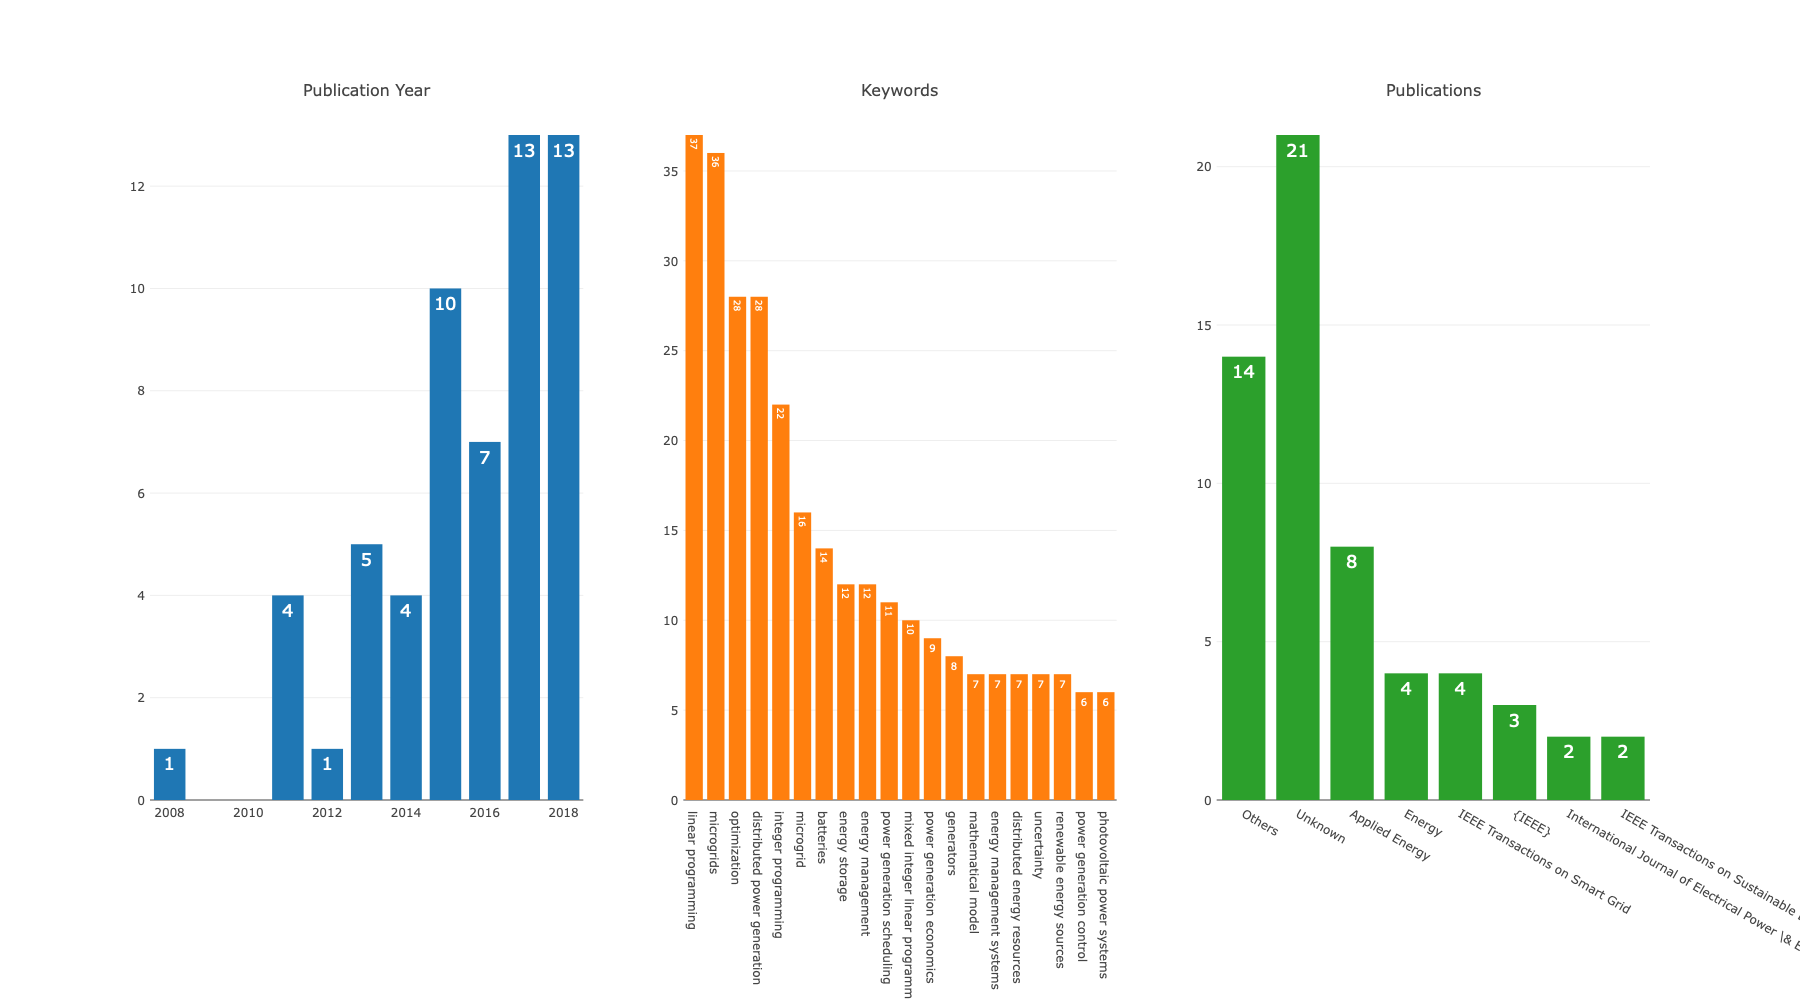
\includegraphics[width=\textwidth]{pictures/Figure_1.png}
	\caption{Results of an automated Descriptive Analysis}
	\label{descriptive_anaylsis_results}
	\flushleft\quad\quad\footnotesize{Source: Own illustration.}
\end{figure}	
Looking at the keywords used to describe the publication shows that, unsurprisingly, the most often occuring keywords are the ones used in conducting the search: 'linear programming', 'microgrids' and 'optimization'. 'distributed energy generation' and 'distributed energy resources'are mentioned 37 times, 'batteries' and 'energy storage' a total of 28 times, and 'renewable energy sources' and 'generators' a total of 16 times. This illustrates the focus on decentralized energy sources and storage, more specifically renewables and small scale combined heat and power generation that prevails throughout the literature.
\\
The publication chart is not very enlightening. This is due to the fact 28 out of 61 publications are conference papers which either appear under others because there is only one instance of that particular conference or unknown. From a more general point of view though almost all papers are published either by Elsevier or IEEE, with very few exceptions.


\subsection{Literature Overview}
The first question in need of an answer in optimizing a microgrids design and dispatch is the question of the modelling approach itself. Although the dataset of literature derived from the methodology described in 2.2 is biased towards Linear Programming, which was one of the search and filter criteria, it contains multiple employed methodologies. For example, \cite{7975049} employ both a Mixed Integer Linear Programming (MILP) model and a Genetic Algorithm (GA) and come to the conclusion that while both deliver accurate and robust results the MILP model is faster. \cite{NEMATI2018944} mostly concur. While in this case, the results of the GA were better in two scenarios, it was outperformed by the MILP model in the remaining three.
A key problem of MILP however seems to be its deterministic nature, which anticipates perfect knowledge of all the parameters involved. Especially for optimisation problems regarding a short timeframe, such as day-ahead scheduling this is a significant problem, since actual parameters may be different. Several methods addressing this problem can be found in literature. 
\\
One such method are rolling time horizons. This approach optimizes the dispatch of a microgrid for a fixed time horizon based on steadily updated forecasts of the uncertain paremeters. The optimization is repeated periodically to reflect the updated forecasts \cite{palma2013microgrid} \cite{silvente2015rolling} and increase dispatch accuracy in the nearer future. Rolling Horizon Optimization is however unfit to optimize investment, since it is not possible to adapt investment decisions ex post to changed conditions.
\\
While the rolling time horizon method helps to limit uncertainty by reacting to changes of input parameters, Robust Optimization and Stochatsic Optimization try to proactively account for a variety of possible scenarios. Robust Optimization achieves this by optimizing for a number of scenarios deemed equally likely, as in \cite{CRAPARO2017135} using ensemble weather forecasts or in \cite{8240914} and \cite{zhang2015optimal} using upper and lower boundaries for uncertain parameters. Stochastic Optimization on the other hand uses detailed probability distributions to weigh the probability of each scenario occuring as explained in \cite{7540870}. To arrive at these distributions secondary tools are usually needed. Shams et al use a simple Gaussian randomization to make their demand data reflect uncertainty, as well as more specific distributions for irridiation and wind speeds. A number of other methodologies appear in literature such as employing a Monte Carlo simulation \cite{ZHENG2018204} or deriving multiple scenarios and corresponding realization probabilities from historical data \cite{7244857}.
\\
The scope of the microgrid models found in literature varies greatly. A constant however is the definition of a microgrid as bounded, operating in a small geographical zone and with a clear electrical boundaries \cite{TAVAKOLI20181}\cite{mashayekhMixedIntegerLinear2017}\cite{7853085}; managing local loads \cite{zhang2013efficient} \cite{ZHENG2018836}; possibly containing various generation units and storage \cite{silvente2015rolling}\cite{7741704} and possibly being able to exchange power with the main grid \cite{NEMATI2018944}\cite{SOLTANINEJADFARSANGI2018257}, from whose perspective it is seen as a single entity \cite{KOLTSAKLIS2018318}.
\\
While most of the selected literature consider cases where a grid connection exists and can be used at all times, there is a number of publications that consider either completely islanded microgrids \cite{ZHANG20181229}\cite{palma2013microgrid} \cite{6872087}\cite{7281564} or microgrids that can sustain themselves in islanded mode for extended periods for exapmle in case of natural disasters \cite{TAVAKOLI20181}.
\\
The clearest distinctions between microgrid models, after the object and applied methodology is properly defined, is based on the aspect or aspects that the model is supposed to optimize. The literature can be split in two groups, either optimizing only dispatch or both investment (e.g. the planning phase) and dispatch. The former group is definitely the larger, with only 12 out of 61 publications considering investment. Notably only one of these \cite{7540870} uses any of the methods to model uncertainty discussed above.
\\
There is also significant diversity in literature when it comes to the technologies considered in modelling.
Modelling dispatchable (eg. non-renewable) as well as non-dispatchable (eg. renewable) generation is rather common, but the specifics differ:
While most models consider PV or Wind as well as a CHP generator, the included generation technologies are as diverse as geothermal generators \cite{7975049} and gas turbines \cite{UMEOZOR2016272} \cite{NEMATI2018944}. In addition to modelling electricity, some publications also consider heat generation and transmission \cite{LAUINGER201624}\cite{wouters2015energy}. This is valuable, because the economic performance of a non-renewable generation unit (usually CHP) present in most models depends heavily on if and how the heat is used, as \cite{costa2014mixed} point out.
\\
The types of storage used in literature also vary. Although battery storage \cite{7399422}\cite{UMEOZOR2016272}\cite{6465822} or an abstract storage device \cite{6669807}\cite{zhang2011optimal} are the most common choices, there are a number of papers modeling heat storage \cite{zhang2013efficient}\cite{zhang2015optimal}\cite{LAUINGER201624}\cite{wouters2015energy}, and some with more exotic technology choices such as flywheels \cite{6700453} or an electrolyzer \cite{7125149}.
\\
In addition to these generation and storage technologies some publications also model the network topology \cite{8023785}\cite{7972908}\cite{SHAMS2018326} and some even consider electrical phenomena such as active and reactive power losses \cite{7741704}\cite{mashayekhMixedIntegerLinear2017} and voltage deviation \cite{7741704}. 
\\
Demand side management, which some models implement is usually represented by dividing loads into different categories. \cite{7972908} distinguish between 'critical loads' ,meaning loads that absolutely have to be satisfied, 'shiftable loads', meaning loads that have to be satisfied, although there is a time window, rather than an exact point in which they can be serviced, and 'adjustable' loads, which can be dropped if needed. Although the terms may vary, and many publications do not introduce the 'shiftable loads' category alltogether, these conceptual distinctions are made by a number of other authors \cite{silvente2015rolling}\cite{zhang2015optimal}\cite{8216436}.
\\
The model results depend almost as much on the given input parameters used in case studies as on the modelling approach itself. There is however only a limited number of publications with detailed documentation of the parameters used.
The used parameters can be broadly categorized as eiter economic parameters, such as capital and operation and maintenance cost for the technologies used, generation related parameters such as irridiation and wind speeds, and load data, representing consumer behaviour.
\\
In publications documenting cost parameters there is a clear trend towards a split of technology cost into investment and maintenance cost. However, whereas \cite{LAUINGER201624} define maintenance cost as a fixed cost per unit of time, \cite{wouters2015energy} define it as a function of kilowatthours produced, a measurement which \cite{LAUINGER201624} call 'fuel costs'. \cite{7399422} choose a definition closer aligned with the former, they however define yearly maintenance cost simply as a flat percentage of the units' investment cost.\cite{KOLTSAKLIS2018318} seem to neglect maintenance costs alltogether focusing only on investment costs. While some models document econimic paramters such as discount rates \cite{7399422}, many don't and it is unclear if future flows of value are properly discounted in these models. Furthermore many of the publications declare cost parameters as assumptions rather than trying to derive them from sources, although a few such as \cite{LAUINGER201624} and \cite{wouters2015energy} do so.
\\
The selected literature offers multiple ways of obtaining input parameters of metereological data. \cite{7981571} use historical metereological data while \cite{palma2013microgrid} build a prediction model for forecasting irridiation and wind speeds. Similarly there are authors who use historical data for load parameters such as \cite{7981571} and ones who generate synthetic data based on appliance use and probabilistic models \cite{zhang2013efficient}\cite{zhang2011optimal}\cite{zhang2015optimal} or neural networks using empirical data \cite{palma2013microgrid}.
\\
When it comes to modelling tools DER-CAM \cite{LAUINGER201624}\cite{ZHENG2018204}\cite{8023785} and HOMER \cite{amrollahi2017techno}\cite{ZHENG2018204}\cite{LAUINGER201624} are the most often referenced. DER-CAM or Distributed Energy Resources Customer Adoption Model is an optimizatioon tool developed at Berkeley Labs and uses Mixed Integer Linear Programming to optimize portfolio, placement, sizing and dispatch of Microgrid Energy Systems \cite{DistributedEnergyResources2018}. HOMER Grid is a commercial optimization tool for behind the meter systems. Its main advantage is it's large database of components and tariff rates in the United States and Canada \cite{HOMERGridBehindtheMeter2018}. The most often mentioned solver is the CPLEX commercial solver \cite{sechilariu2014supervision}\cite{NEMATI2018944}\cite{UMEOZOR2016672}\cite{7741704}... . Most of the models are written in GAMS \cite{silvente2015rolling}\cite{UMEOZOR2016672}\cite{CRAPARO2017135}..., although many are written in MATLAB \cite{7741704}\cite{7972908}... .
\\
Open source tools seem scarcely available. A search of 'microgrid optimization' on github.com, the major open source software platform, brings up only 3 items with more than one star, none of them has more than ten (popular libraries might have thousands)\cite{GithubSearchMicrogrid2018}. The most up-to-date one has not been updated for a year and none features a graphical user interface.

\newpage
\section{Model}

\subsection{Time}
The range of scenarios and complexity the model can handle is, among other things, dependant on its implementation of discrete time. More and smaller timesteps and a representative sample of diverse expectable conditions regarding the parameters leads to higher model accuracy. Of course the amount of timesteps is limited by processing power and therefore by model complexity. To enable both diverse and therefore potentially discountinous parameter sets and a reasonable length for each set, the length of 1 hour is chosen for the basic timestep 
$t; t \in [1,T]; T \in \mathbb{N} ;$. $T$ denotes the number of hours in each disontinous sets of supply and demand parameters.
Furthermore the ability of including multiple discontinous sets of supply and demand parameters of the same length in one scenario is gained by introducing a second iterator 
$s; s \in [1,S]; S \in \mathbb{N} ;$. $S$ denotes the number of discontinous sets of supply and demand parameters.





\subsection{Households}
To properly conduct trading and for the future possibility of adding voltage and topological constraints to the model, the households are modeled as independent entities, each with its own demand, generation and storage. Therefore a third iterator $u; u \in [1,U]; U \in \mathbb{N};$ is introduced. $U$ denotes the number of households modeled.
An absract household $H$ is defined as a tuple of storage and generation devices as well as demand curves. For discrete storage and generation devices two seperate sets of positive integers define how much of each option available in the scenario was installed. Additionally each household has a price $shiftP$ and $curtP$ at which they are willing to shift or curtail a unit  of their load respectively.
\begin{equation}
	H := (GEN, ST, dGEN, dST, DEM, shiftP, curtP)
\end{equation}

A conrete household $H_u$ implements these values:
\begin{equation}
	GEN \in \mathbb{R}^{K}; GEN_k \geq 0 \forall k; k\in [0,K]
\end{equation}
\begin{equation}
	ST \in \mathbb{R}^{L}; ST_l \geq 0 \forall l; l\in [0,L] 
\end{equation}
\begin{equation}
	dGEN \in \mathbb{N}^{M}
\end{equation}
\begin{equation}
	dST \in \mathbb{N}^{N}
\end{equation}
with\\
$k,K,L,l,M,N \in \mathbb{N}$\\
and\\
$shiftP, curtP \geq 0$

$K$ and $L$ denote the amount of generation and storage devices in household $H_u$.This, in practice, is equal to the amount of linear scaling investment options for each category, since a zero capacity device is still modeled as a device. $M$ and $N$ denote the amount of discrete investment options in their respective category. $GEN_k$ and $ST_l$ are the capacities installed of the k-th and l-th linear investment option respectively. $GEN_m$ and $dST_n$ are the amount installed of the m-th and n-th discrete investment option available. $DEM$ is further defined in the subsection demand.





\subsection{Internal Variables}
The objective of the model is to find optimal investment, dispatch and trade. Therefore, the following sets of internal paramters are introduced:
	\\
	$\forall u,k,l,m,n,s,t$:
	\\
	\begin{equation}
		toTR_{u,s,t}, fromTR_{u,s,t} \geq 0
	\end{equation}
	
	\begin{equation}
		genS_{u,k,s,t}, dgenS_{u,m,s,t}, fromST_{u,l,s,t}, toST_{u,l,s,t}, fromDST{u,n,s,t}, toDST{u,n,s,t} \geq 0
	\end{equation}
	
	\begin{equation}
		toSC{u,s,t}, fromSC{u,s,t}, fromGR{u,s,t}, toGR{u,s,t}, ncS_{u,s,t},  \geq 0
	\end{equation}
	\\
	$\forall u,k$:
	\begin{equation}
		H_u->GEN_k \geq 0
	\end{equation}
	\\
	$\forall u,l$:
	\begin{equation}
		H_u->ST_l \geq 0
	\end{equation}
	
	$\forall u,m$
	\begin{equation}
		H_u->dGEN_m \in \mathbb{N}
	\end{equation}
	
	$\forall u,n$
	\begin{equation}
		H_u->dST_n \in \mathbb{N}
	\end{equation}





\subsection{Generation}
\todo{Introductory sentence generation}\\
Therefore an abstract linear generation device $GEN$ and an abstract discrete generation device $dGEN$, which can represent a range of technology options, are defined:\\
	\begin{equation}
		GEN := (C_{Cap}, C_{OpFix}, C_{OpVar}, T_{Life}, EFF_{el}, PR, minFl)
	\end{equation}
	\begin{equation}
		dGEN := (CAP, C_{Cap}, C_{OpFix}, C_{OpVar}, T_{Life}, EFF_{el}, PR, minFl)
	\end{equation}
	$CAP \geq 0$, which is only required for discrete investments, defines the generation capacity of the discrete investment option.
	$C_{Cap} \geq 0$ defines the total investment cost for discrete generation devices. For linear generation devices the investment cost is expressed in terms of one unit of capacity.
	$C_{OpFix} \geq 0$ expresses the fixed maintenance cost per unit of time.
	$C_{OpVar} \geq 0$ expresses the variable maintenance cost per unit of input consumed.
	$T_{Life} \in \mathbb{N}$ defines the life expectancy of a generation device, e.g the time before it is replaced. 
	$EFF_{el} \in [0,1]$ defines the ratio of supplied energy, for example sunlight or gas, to produced electricty.
	$PR \in [0,1]$ is another definable penalty to electricity production, which can, for example, express the degradation of solar cells. 	
	$minFl \in [0,1]$ denotes the minimal possible electricity production as a percentage of capacity.





\subsection{Storage}
The introduction of the concept of energy storage is necessary if the use of a large proportion of intermittent power production while maintaining intermittent power demand is to be seriously explored.
Therefore an abstract linear storage device $ST$ and an abstract discrete storage device $dST$, which can represent a range of technology options, are defined:\\
	\begin{equation}
		ST := (C_{Cap}, T_{Life}, EFF_{+-}, LOC_{1h}, maxP_{+}, maxP_{-})
	\end{equation}
	\begin{equation}
		dST := (CAP, C_{Cap}, T_{Life}, EFF_{+-}, LOC_{1h}, maxP_{+}, maxP_{-})
	\end{equation}
	$CAP \geq 0$, which is only required for discrete investments, defines the usable capacity of the discrete investment option.
	$C_{Cap} \geq 0$ defines the total investment cost for discrete storage devices. For linear storage investment options the investment cost is expressed in terms of one unit of capacity.
	$T_{Life} \in \mathbb{N}$ defines the life expectancy of a storage device, e.g the time before it is replaced. To be able to better estimate this value it is assumed, that storage is, on average, cycled once per day.
	$EFF_{+-} \in [0,1]$ defines the roundtrip efficiency, e.g. what proportion of one unit of power is left after charging and discharching inefficiencies. It is used to compute the charge and discharge efficiencies.
	The charge efficiency $EFF_{+}$ is defined as $EFF_{+} = \sqrt{EFF_{+-}}$ and the discharge efficiency $EFF_{-}$ as $EFF_{-} = 1/EFF_{+}$.\\
	$LOC_{1h} \in [0,1]$ expresses the relative amount of charge lost, during one timestep of storage.
	$maxP_{+} \geq 0$ and $maxP_{-} \geq 0$ denote the maximum charge rate and discharge rate respectively.





\subsection{Trade}
Trade is implemented as an exchange platform, which sums up deposits and withdrawals of power at each timestep and always needs to be balanced. This approach has the advantage of reducing the number of constraints and therefore complexity greatly, although it is not very well suited to handle grid topology constraints which might be addded in the future.\\
The trade constraint is defined as:
\\

$\forall s,t$
\begin{equation}
	\sum_{u = 1}^{U}{toTR_{u,s,t}-fromTR_{u,s,t}} = 0
\end{equation}





\subsection{Demand}
Abstract demand data $DEM$ is defined as a set of the size $S$ of demand profile sets of the size $T$:
\begin{equation}
 DEM:= \{DEM_s | s \in [1,S]; s\in \mathbb{N}; \forall DEM_s, DEM_s := \{DEM_{s,t} | t\in [0,T]; t \in \mathbb{N}\}
\end{equation}

As frequently applied in literature, $DEM_{s,t}$ is not a demand value, but rather a tuple of three demand values, critical demand, shiftable demand and curtailable demand \cite{silvente2015rolling}\cite{zhang2015optimal}\cite{8216436}\cite{7972908} : 
\begin{equation}
 DEM_{s,t}:= (critDEM_{s,t}, shiftDEM_{s,t}, curtDEM_{s,t}) 
\end{equation}

$\forall s,t$\\
$critDEM_{s,t}, shiftDEM_{s,t}, curtDEM{s,t} \geq 0$

Critical demand will be met by the model as it is seen as a constraint. Shiftable demand can be shifted by one hour at a fixed rate defined for each household. Curtailable demand can be dropped at a fixed rate defined for each household.





\subsection{Grid}
The modeled microgrid is connected to the grid via a common point of coupling. The grid is defined as:

\begin{equation}
	GRID:= (maxS, maxD, gridC, feedC)
\end{equation}\\
with\\
$maxS,maxD, gridC, feedC \in \mathbb{R}^{S \times T}$\\
and $\forall s \in [1,S], t \in [1,T]; s,t \in \mathbb{N}$: \\
$maxS{s,t}, maxD{s,t}, gridC{s,t}, feedC{s,t} \geq 0$

$maxS$ describes the maximum amount of power supplied by the grid at each timestep $(s,t)$, while $gridC_{s,t}$ expresses the price at which this power can be bought.
$maxD$ describes the maximum amount power that can be fed into the the grid at timestep $(s,t)$, while $feedC_{s,t}$ expresses the price at which the grid buys this power. 





\subsection{Power Balance}
The power balance constraint describes the need for a balance between supply and demand at each node at each timestep: \\

$\forall u,t,s$:
\begin{equation}
	\begin{split}
		H_u->critDEM_{s,t} + H_u->shiftDEM_{s,t} + H_u->curtDEM{s,t}\\
		= \\
		fromGR_{u,s,t} - toGR{u,s,t} + \sum_{k=1}^K{genS_{u,k,s,t}} + \sum_{m=1}^M{genS_{u,m,s,t}} \\ 
		+ fromTR{u,s,t} - toTR{u,s,t} + scS_{u,s,t} - scS_{i,s,t-1} + ncS_{u,s,t} \\
		+ \sum_{l=1}^L{fromST_{u,l,s,t} - toST_{u,l,s,t}} + \sum_{n=1}^N{fromDST_{u,n,s,t}-toDST_{u,n,s,t}}
	\end{split}
\end{equation}

\todo{explain this calculation}




\subsection{Cost Minimization Formula}
The cost minimization formula calculates the cost of all investment and dispatch decisions made:
\begin{equation}
	\min C_{total} = C_{Investment} + C_{Dispatch}
\end{equation}
\begin{equation}
	\begin{split}
		C_{Investment} = \sum_{u=1}^{U}[\sum_{k=1}^K{(GEN_k->C_{Cap} * H_u->GEN_k)}\\
		+ \sum_{l=1}^L{(ST_l->C_{Cap} * H_u->ST_l)}\\
		+ \sum_{m=1}^M{(dGEN_m->C_{Cap} * H_u->dGEN_m)}\\
		+ \sum_{n=1}^N{(dST_n->C_{Cap} * H_u->dST_n)}]
	\end{split}
\end{equation}

\todo{explain this calculation}
\begin{equation}
	\begin{split}
		C_{Dispatch} = \sum_{s=1}^{S}\sum_{t=1}^{T}\sum_{u=1}^{N}(gridC_{s,t} * fromGR_{u,s,t} - feedC_{s,t} * toGR{u,s,t}\\
		+ H_u->curtP * ncS_{u,s,t} + H_u->shiftP * scS{u,s,t})
	\end{split}
\end{equation}

\todo{explain this calculation}


	\section*{Constraints}
	
	\begin{equation}
		S_{PV_i,t,y} = SF_{t,y} * CP_{PV_i}
	\end{equation}
	 
	 \begin{equation}
	 		S_{SC_{i,T,Y}} = 0 
	 \end{equation}
	
	 \begin{equation}
	 		S_{TS_{i,T,Y}} = 0 
	 \end{equation}
	
	 \begin{equation}
	 		S_{TS_{i,t,y}} \leq  CP_{ST_i}
	 \end{equation}


\newpage
\section{Case Study}
\subsection{Meterological Data}
Hourly irridiation data (in $KWm^{-2}$) for <<PLACE>> is sourced from \cite{pfenningerLongtermPatternsEuropean2016}. 
\subsection{Investment Options}
\begin{table}[H]
	\centering
	\caption{Parameters describing the conversion technologies}
	\begin{tabular}{lllll}
		\hline
		\textbf{Parameter}			& \textbf{Name}			& \textbf{Unit}			& \textbf{Value}	&\textbf{Reference}     \\ \hline
		\textit{Photovoltaic System} & & & &\\
		Installation Cost           & information     		& \euro $KW^{-1}$  		& 1300				& Estimate based on \cite{wirthAktuelleFaktenZur2018}, \cite{SolarmoduleEBay2018}, \cite{ModulePriceIndex2018}   \\
		Maintenance Cost            & information     		& \euro $KW^{-1}yr^{-1}$& 50				& Estimate \\
		Lifetime                    & information     		& $yr$  				& 25 				& \cite{wirthAktuelleFaktenZur2018}   \\
		Electric Efficiency         & information     		& $\%$  				& 17				& \cite{wirthAktuelleFaktenZur2018}   \\
		Performance Ratio           & information     		& $\%$  				& 85				& \cite{wirthAktuelleFaktenZur2018}   \\
		\textit{CHP Micro Fuel Cell} & & & &\\
		Installation Cost           & information     		& \euro $KW^{-1}$  		& 3500 				& Estimate based on \cite{LAUINGER201624}    \\
		Maintenance Cost            & information     		& \euro $KW^{-1}yr^{-1}$& 175				& Estimate based on \cite{LAUINGER201624}   \\
		Fuel	 Cost           			& information     		& \euro $KWh^{-1}$   	& 0,0608			& \cite{NaturalGasPrices2018}   \\
		Lifetime                    & information     		& $yr$  				& 15 				& \cite{LAUINGER201624}    \\
		Electric Efficiency         & information     		& $\%$  				& 60				& \cite{BlueGENWorldsMost2018}   \\
		Thermal Efficiency			& information     		& $\%$  				& 21				& \cite{BlueGENWorldsMost2018}   \\
		Minimum Gas Flow    			& information     		& $\%$ 		 			& 30				& \cite{LAUINGER201624}   \\
		\hline
	\end{tabular}
\end{table}

\begin{table}[H]
	\centering
	\caption{Parameters describing the storage technologies}
	\begin{tabular}{lllll}
		\hline
		\textbf{Parameter}			& \textbf{Name}			& \textbf{Unit}			& \textbf{Value}	&\textbf{Reference}     \\ \hline
		\textit{Li-Ion Battery 1} & & & &\textit{Tesla Powerwall} \\
		Installation Cost              & information     	& \euro 				& 10000				& Estimate based on \cite{PowerwallTesla2018}   \\
		Usable Capacity				   & information 		& $KWh$ 				& 13.5 				& \cite{PowerwallTesla2018} 	\\
		Lifetime			               & information     	& $yr$  				& 10 				& Estimate based on \cite{PowerwallTesla2018} \\
		Roundtrip Efficiency           & information     	& $\%$  				& 90				& \cite{PowerwallTesla2018}   \\
		Self-Discharge		           & information     	& $\%hr^{-1}$  			& 5					& \cite{LAUINGER201624}   \\	
		Max. charging power            & information    	& $kW$  				& 4.6 				& \cite{PowerwallTesla2018}      \\
		Max. discharging power         & information     	& $kW$   				& 4.6 				& \cite{PowerwallTesla2018}      \\
		Initial State of Charge        & information     	& $\%$  				& 100 				& Assumption   \\
		Terminal State of Charge       & information     	& $\%$  				& 100 				& Assumption   \\
		
		\textit{Li-Ion Battery 2} & & & & \textit{Victron Energy Lithium HE Batterie} \\
		Installation Cost              & information     	& \euro  				& 5000				& Estimate based on \cite{VictronEnergyLithium2018}   \\
		Usable Capacity				   & information 		& $KWh$ 				& 4 				& based on \cite{LithiumIonenHEHigh2018} considering maximum depth of discharge\\
		Lifetime			               & information     	& $yr$  				& 10 				& Estimate based on \cite{LithiumIonenHEHigh2018}   \\
		Roundtrip Efficiency           & information     	& $\%$  				& 92 				& \cite{LAUINGER201624}    \\
		Self-Discharge		           & information     	& $\%hr^{-1}$  			& 5					& \cite{LAUINGER201624}   \\	
		Max. charging power            & information    	& $KW$  				& 4.8				& \cite{LithiumIonenHEHigh2018}    \\
		Max. discharging power         & information     	& $KW$   				& 7.2				& \cite{LithiumIonenHEHigh2018}    \\
		Initial State of Charge        & information     	& $\%$  				& 100 				& Assumption	   \\
		Terminal State of Charge       & information     	& $\%$  				& 100 				& Assumption   \\	
		\hline
	\end{tabular}
\end{table}

\subsection{Further Assumptions}

\begin{table}[H]
	\centering
	\caption{Further Assumed Parameters}
	\begin{tabular}{lllll}
		\hline
		\textbf{Parameter}			& \textbf{Name}			& \textbf{Unit}			& \textbf{Value}			&\textbf{Reference}     \\ \hline
		Discount Rate              	& information     		& $\% yr^{-1}$  		& 1.5						& Estimate   \\
		-----			            & information     		& information  			& &    \\
		-----					    & information     		& information  			& &    \\		
		\hline
	\end{tabular}
\end{table}


\newpage
\section{Results and Discussion}
\newpage


\section{Appendix}
\subsection{Literature Review}
The used search String was:  [microgrid AND (optimization OR opimisation) AND linear programming]
\\
The used databases are ScienceDirect, IEEE Xplore and Google Scholar.
\\
The original dataset consistet of 300 publication of which 275 remained after duplicates where merged.
\\
The search string for the Abstract Keyword Search was [(microgrid OR micro-grid OR off-grid) AND (optimization OR optimisation OR optimise OR optimal OR optimally) AND (linear programming OR linear program OR mixed integer)
\\
After the abstract keyword search was conducted 106 publications remained.
\\
The inclusion criteria were:
\begin{enumerate}
	\item An optimization model is employed.
	\item There is some discussion about the design of the model.
	\item The objective of the model is the optimization of design or dispatch of a single microgrid.
	\item There is some sort of case study conducted.
\end{enumerate}
The exclusion criteria were:
\begin{enumerate}
	\item The publication is not in English language.
	\item The full text is not obtainable for this author with reasonable effort.
	\item The publication is a Work-In-Progress / Conference Paper version of a publication published in a journal and also included in this dataset.
	\item The mathematical model designed is non-linear.
	\item The mathematical model designed only considers a specific aspect of dispatch or design, not the entirety.
	\item The mathematical model is mostly focused on heat generation/distribution rather than electricity.
\end{enumerate}
After the filtering by inclusion and exclusion criteria 58 publications remained.

% weitere Dokumente einfügen mit den gleichen zwei Befehlen

%\nocite{*}									% gibt zum Testen des Literaturverzeichnisses alle Bibeinträge aus
\chead{\textit{References}}				    % siehe oben 
\renewcommand\refname{Literature}			% in Literaturverzeichnis umbenennen
\printbibliography
%[heading=bibintoc]
\end{document}
